 %% 
%% ACS project dissertation template. 
%% 
%% Currently designed for printing two-sided, but if you prefer to 
%% print single-sided just remove ",twoside,openright" from the 
%% \documentclass[] line below. 
%%
%%
%%   SMH, May 2010. 


\documentclass[a4paper,12pt]{report}


%%
%% EDIT THE BELOW TO CUSTOMIZE
%%

\def\authorname{Sumaiyah Y.\ Kola\xspace}
\def\authorcollege{Clare College\xspace}
\def\authoremail{sk940@cam.ac.uk}
\def\dissertationtitle{Exploring Mechanisms for Uncovering the Misuse of AI as a Service}
\def\wordcount{TODO}


%\usepackage[dvips]{epsfig,graphics} 
\usepackage{epsfig,graphicx,verbatim,parskip,tabularx,setspace,xspace,hyperref}
% Pseudocode for algorithms
\usepackage{algorithmicx}
\usepackage[ruled]{algorithm}
\usepackage{algpseudocode}
% subfigures
\usepackage{subcaption}
% tables
\usepackage[normalem]{ulem}
\useunder{\uline}{\ul}{}
% arg max
\usepackage{amsmath}
\DeclareMathOperator*{\argmax}{arg\,max}


%% START OF DOCUMENT
\begin{document}
	
	
	%% FRONTMATTER (TITLE PAGE, DECLARATION, ABSTRACT, ETC) 
	\pagestyle{empty}
	\singlespacing
	% title page information
\begin{titlepage} 

\begin{center}
\noindent
\huge
\dissertationtitle \\
\vspace*{\stretch{1}}
\end{center}

\begin{center}
\noindent
\huge
\authorname \\
\Large
\authorcollege      \\[24pt]
%\begin{figure}

\includegraphics{CUni3.pdf}
%\end{figure}
\end{center}

\vspace{24pt} 

\begin{center}
\noindent
\large
{\it A dissertation submitted to the University of Cambridge \\ 
in partial fulfilment of the requirements for the degree of \\ 
Master of Engineering in Advanced Computer Science} 
\vspace*{\stretch{1}}
\end{center}

\begin{center}
\noindent
University of Cambridge \\
Computer Laboratory     \\
William Gates Building  \\
15 JJ Thomson Avenue    \\
Cambridge CB3 0FD       \\
{\sc United Kingdom}    \\
\end{center}

\begin{center}
\noindent
Email: \authoremail \\
\end{center}

\begin{center}
\noindent
\today
\end{center}

\end{titlepage} 

\newpage
\vspace*{\fill}

	\onehalfspacing
	\newpage
{\Huge \bf Declaration}

\vspace{24pt} 

I \authorname of \authorcollege, being a candidate for the Part III in
Advanced Computer Science, hereby declare that this report and the
work described in it are my own work, unaided except as may be
specified below, and that the report does not contain material that
has already been used to any substantial extent for a comparable
purpose.

\vspace{24pt}
Total word count: \wordcount

\vspace{60pt}
\textbf{Signed}: 

\vspace{12pt}
\textbf{Date}:


\vfill

This dissertation is copyright \copyright 2010 \authorname. 
\\
All trademarks used in this dissertation are hereby acknowledged.



\newpage
\vspace*{\fill}

	\singlespacing
	\newpage
{\Huge \bf Abstract}
\vspace{24pt} 


\textbf{TODO}

\newpage
\vspace*{\fill}

	
	\pagenumbering{roman}
	\setcounter{page}{0}
	\pagestyle{plain}
	\tableofcontents
	\listoffigures
	\listoftables
	
	\onehalfspacing
	
	%% START OF MAIN TEXT 
	
	%\chapter{Introduction}
	\chapter{Introduction}
	\pagenumbering{arabic} 
	\setcounter{page}{1} 
	
	\section{Motivation}
	
	\section{Related Work}
	
	\section{Key Contributions}
	
	\section{Summary}
	The project is driven by the fact that numerous generic pre-built AI models are available as a service, on-demand. Integrating AI functionality into applications is now easier than ever. Consequently…lots of potential for misuse
	% 3-4 sentences just summarising intro/motivation
	
	
	\chapter{Real World Data}
	From facial recognition and speech translation to content moderation and medical transcriptions, AIaaS providers offer functionality for a vast range of generic and specialised applications. Given the variety of services available, it may be impractical for service providers to run misuse indicators for all possible scenarios, in the first instance. Understanding general patterns of customer behaviour can greatly assist AIaaS providers in deciding where further investigation is required. 
	
	\section{Motivation}
	
	AIaaS platforms already generate (log) information about their service usage \cite{shahrad2020serverless}. Providers often charge for services per use and the usage logs are used to support billing, among other things. The transaction data can help in identifying patterns of customer behaviour and identifying potential misuse.
	
	\textbf{TODO: mention existing approaches e.g. Bank fraud and NID}
	
	The aim of this misuse indicator is to provide insights regarding the landscape of customer behaviour, and flag areas that may warrant further attention. We examine the use of clustering approaches to group customer behaviour, highlighting common habits and patterns and identifying any anomalous ones. 
	
	\section{Approach}
	Outlier detection is the process of identifying unusual patterns of behaviour or rare occurrences that raise suspicions as they differ substantially from the rest of the data. We consider a generic, exploratory approach, searching for different classes of behaviour in real-world data and identifying potential outliers. 
	
	This task involves generating realistic traces of AIaaS data, from analogous datasets, to 
	indicate possible scenarios of misuse. Then, using cluster analysis based detection models, we formulate methods for uncovering the potential misuse. Examining a dataset that reflects real consumer behaviour would be useful for this study.
	
	\section{Data}
	While there is a lack of publicly accessible data (usage logs) from AIaaS providers, a dataset containing real-world usage data has recently been made public by Microsoft \cite{shahrad2020serverless}. It contains customer usage of Microsoft’s Azure Function as a Service (FaaS). Similar to AIaaS, FaaS also involves invoking specific functions through a web-based API. As such, in terms of mapping a usage landscape that is grounded in reality, we may consider this dataset reasonably analogous to AIaaS customer usage. 
	
	The dataset contains real-world customer metadata over a period of 14 days between July 15th and July 28th, 2019. Each customer can be associated with one or applications and each application is associated with one or more function calls. For each day, the dataset includes the:
	\begin{itemize}
		\item Function invocation count (FIC), per function, per minute over 24 hours.
		\item Function execution duration (FED), per function. The data is averaged and presented as a set of weighted percentiles and summary statistics over 24 hours.
		\item Application memory allocation (AMA), per application. The data is averaged and presented as a set of weighted percentiles and summary statistics over 24 hours.
	\end{itemize}
	A full schema of the dataset can be found here \cite{AzurePub78:online}.
	
	\subsection{Preprocessing}
	The FED and AMA data are provided as a set of weighted percentiles every 24 hours that indicate a probability distribution. The first step in preprocessing is to regenerate representative FED and AMA data at minute level granularity with the given data.
	
	The FED is provided, per function, as a set of percentiles and summary statistics over 24 hours. We assume that the data has a normal distribution. In order to sample this distribution the mean and standard deviation is required. Although the summary statistics for FED provide the mean for each function call, they do not include the standard deviation. Fortunately, the standard deviation may be estimated using known heuristics and the data given.
	
	The empirical, or three-sigma rule, claims that nearly all values lie within three standard deviations of the mean. In particular, it predicts that 68\% of observations falls within the first standard deviation $(\mu \pm \sigma)$, $95\%$ within the first two standard deviations $(\mu \pm 2\sigma)$, and $99.7\%$ within the first three standard deviations $(\mu \pm 3\sigma)$. We can compute an approximation for the standard deviation by substituting in the cumulative percentages, or percentiles. This process is repeated on the AMA dataset. 
	
	The FIC, FED and AMA data is standardised. To allow categorical attributes to be understandable to models, they are numerically encoded. The remaining numerical features are log normalised so that attributes have similar magnitudes. This prevents features with larger values from carrying more significance in the network.
	
	
	\section{Clustering Approaches}
	In order to group different types of behaviour and identify potential outliers, we analyse the usage logs with clustering. There are a wide variety of clustering algorithms that have significantly different ideas about what defines a cluster and how to effectively identity clusters. In this section we compare and evaluate the performance of three clustering algorithms, namely DBScan, Gaussian mixture models and $k$-means. 
	
	\subsection{$k$-means}
	$k$-means is an extensively used, centroid-based machine learning algorithm that aims to partition the data into $k$ clusters. Each cluster is associated with its center, or `centroid’. A cluster centroid is the arithmetic mean of all the points belonging to that cluster. Optimal clustering with $k$-means is achieved when each point is closer to its own cluster centroid than any other centroid. 
	
	Initially, the cluster centroids are randomly selected. The positions of the centroids are then iteratively optimised until either the positions stabilise or the defined number of iterations is reached.
	
	\subsection{Gaussian Mixture Model}
	A Gaussian mixture model (GMMs) attempts to find a mixture of $k$ Gaussian probability distributions that best model the dataset. As before, $k$ is a predetermined number of clusters. A different Gaussian distribution is used to model each cluster. A GMM uses an expectation-maximisation approach.
	
	GMM addresses two main practical concerns faced by k-means.
	Unlike k-means clustering where each cluster is associated with a hard-edged sphere, \textbf{TODO finish!!} % https://jakevdp.github.io/PythonDataScienceHandbook/05.12-gaussian-mixtures.html 
	
	\subsection{DBScan}
	\label{section:dbscan}
	The Density-based spatial clustering of applications with noise (DBSCAN) algorithm groups together points based on a measurement of distance and a specified minimum number of points \cite{ester1996density}. DBScan can successfully discover clusters of different shapes and sizes from large noisy datasets with outliers. The DBScan algorithm requires the definition of two parameters:
	$Min\_points$:
	epsilon ($\epsilon$): 
	
	and will independently determine the number of clusters. DBSCAN works by determining whether the minimum number of points are close enough to one another to be considered part of a single cluster. Since $\epsilon$ is a fixed value for the maximum distance between two points in a dense region, the algorithm is very sensitive to scale.\textbf{TODO: how to pick parameter vals}  % https://www.analyticsvidhya.com/blog/2020/10/a-simple-explanation-of-k-means-clustering/
	
	\section{Summary}
	% 3-4 sentences just summarising section
	
	
	\chapter{Surveillance Detection}
	Facial recognition is a popular computer vision task that involves recognising and verifying an individual from a photograph of their face. Many of the major AIaaS providers offer products to seamlessly detect, identify and even analyse faces. Facial recognition software however, raises major concerns about privacy and the enabling of mass surveillance. For this task we consider the potential for misuse in the context of processing images of human faces. 
	
	\section{Motivation}
	When it comes to privacy, the misuse of facial recognition technologies is a huge issue. The use of these technologies for potential mass surveillance is raising concerns among the public \cite{gates2011our}. By leveraging the large volume of data available to them, the major AIaaS providers are able to provide highly precise computer vision models, at a low cost. Given the new, lower, barrier to entry, anyone can build a facial recognition application, increasing the risk of misuse. 
	
	In June 2020 after many concerns that the technology was being used to promote racism, IBM announced that it would no longer develop or sell facial recognition software \cite{IBMsaysi68}. The concerns were legitimate; the majority of facial recognition algorithms performed poorly on non-white faces, according to a report from the US National Institute of Standards and Technology \cite{NISTStud33:online}. Notably, not long after IBM, Amazon announced that they would impose a one-year ban on police use of Rekognition \cite{Weareimp80:online}, their cloud-based computer vision platform. Microsoft revealed the following day that they too would stop supplying this software to police forces until the technology is regulated by federal legislation \cite{greene2020microsoft}. The misuse of facial recognition software is easy to imagine, and the high-profile reaction to law enforcement use of face services demonstrates that the concerns are real.
	
	The specifics of the misuse of facial analysis software in other circumstances are yet to be explored. As a result, the illustrative examples we present aim to illustrate and explore specific concerns. In this chapter we explore two potential misuse indicators in the facial recognition domain. The first considers the possibility of large-scale monitoring, or surveillance, while the second considers the possibility of stalking an individual.
	
	\section{Approach}
	The misuse indicators we discuss in this project are not definitive of misuse. Instead, the purpose is to attract the attention of the service provider to specific customer behaviours that may warrant further review. Through this task, we aim to demonstrate the potential of two trait-based indicators. We also highlight the practical overhead considerations of the different approaches available.
	
	In this task, the misuse indicators examine the potential usage logs of a facial recognition service. The usage logs describe the information gathered as a byproduct of using an AIaaS face service. As such each entry in the log file is a vector encoded representation of the face in each image. As face embeddings are vectors, we can easily interpret them as points in the Cartesian coordinate system. For two images of the same person, the distance between the encoding vectors will be small; for different individuals, the distance will be larger \cite{schroff2015facenet}.
	
	A typical usage log would contain a large number of unlabeled faces. Cluster analysis is useful for exploring and grouping a large collection of unlabelled data. We explore the use of clustering algorithms to group the images into the individual identities present in the data. Although the problem of clustering has been extensively explored in pattern recognition, machine learning and statistical scenarios \cite{jain2010data}, it is still relatively recent in the field of face recognition. 
	
	Otto et al. provide a brief review of clustering face images by identity \cite{otto2017clustering}. According to the authors, since there is no universal face representation or distance metric, the performance of a clustering algorithm in this scenario is dependent on the clustering algorithm chosen as well as the quality of the underlying face representation. The chosen face representation is described in section \ref{subsection:preprocessing} while the clustering algorithms are discussed in section \ref{section:clustering_approaches}.
	
	\section{Clustering Approaches}
	\label{section:clustering_approaches}
	The usage logs we examine describe the information gathered as a byproduct of using an AIaaS face service and contain a large number of unlabelled face images. Our aim is to identify the individual identities present in the data. Unfortunately, for the majority of clustering algorithms, the number of clusters must be specified as an input parameter. As we want to independently discover the number of clusters, we explore two alternative clustering methods, namely DBScan and Chinese Whispers, that are explained below. 
	
	\subsection{DBScan}
	DBScan is one of the most widely used density-based clustering algorithms and has proved useful for imaging tasks \cite{dhanachandra2017survey}. A full explanation of DBScan can be seen earlier in section \ref{section:dbscan}. A Euclidean distance metric is used to determine whether two images are likely of the same person. Here $\epsilon$ describes the maximum distance between two face encodings that can be considered the same person. The $minPoints$ parameter states the minimum number of points required to form a dense region. Given that the the dataset includes several people with only one image, we set $minPoints=1$ 
	
	\subsection{Chinese Whispers}
	Chinese whispers (CW) is a hard partitioning, randomised, flat graph-clustering algorithm that works on undirected graphs \cite{biemann2006chinese}. It is an efficient algorithm with a time complexity that is linear in the number of edges. As such, the algorithm is suitable for very large graphs. A graph represents objects and their relations. Instead of using a distance metric, the similarity between objects is encoded in the edges of the graph. 
	
	The CW algorithm begins with every node in the graph assigned to a distinct class with one node in each class. Nodes are then repeatedly chosen randomly, and assigned the ‘strongest’ class in their neighbourhood. The strongest class is the class whose total edge weights to the current node is the largest. In the case of a tie, one class is randomly selected. Once the process converges, or the predetermined number of iterations is reached, the algorithm is complete and the emerging classes represent the network clusters. 
	
	Although the CW algorithm is most frequently used in the field of NLP \cite{di2013clustering}, it is starting to be implemented for computer vision task. Recently, Klip used the algorithm to group images of faces by identity for a forensic investigation task \cite{klip2019fuzzy}. In section \ref{subsection:preprocessing} we describe how we transform the log of images into an undirected weighted graph.
	
	\section{Experimental Setup}
	We conduct two main experiments to explore the potential for clustering faces. The experiments were conducted using the High Performance Computing Service (HPCS). Each experiment was conducted five times, the results averaged.
	
	\subsection{Datasets}
	\label{subsection:datasets}
	To explore the potential of the misuse indicators described, we outline several experiments leveraging three public datasets:
	\begin{itemize}
		\item A subset of the CelebA dataset \cite{liu2015faceattributes}: comprising 40995 face images from 2000 individuals.
		\item ColorFeret by NIST: comprising 11338 face images from 994 individuals \cite{phillips1998feret}.
		\item Labeled Faces in the Wild (LFW): comprising 13233 face images from 5749 individuals \cite{LFWTech}. 
	\end{itemize}
	
	There is only one face in each image. We use CelebA to tune the parameters of the clustering algorithms (see section \ref{subsection:hyper_tuning}). The ColorFeret and LFW datasets are then used to generate the usage logs and evaluate the performance of the clustering algorithms (see section TODO). 
	
	\subsection{Preprocessing}
	\label{subsection:preprocessing}
	Face detection is required prior to face recognition. We use an implementation of the Multi-Task Cascaded Convolutional Neural Network (MTCNN) for face detection and a TensorFlow implementation of FaceNet to generate an embedding for each detected face \cite{davidsan69:online}. 
	
	\subsubsection{Face Detection}
	Face detection is the process of automatically identifying and localising a human face in an image by drawing a bounding box around the extent. We use an implementation of MTCNN, a state-of-the-art deep learning model for face detection based on a paper from Zhang et al. \cite{DBLP:journals/corr/ZhangZL016}.
	
	\subsubsection{Face Recognition}
	FaceNet uses a deep convolutional neural network to extract high quality features from an image of a face \cite{schroff2015facenet}. The facial recognition system takes an image as input and returns a vector of size 128. FaceNet essentially extracts the important features and compresses the image into an embedding. Here we use a pre-trained Keras FaceNet model \cite{nyokimtl39:online} trained on the large MS-Celeb-1M dataset \cite{Guo2016MSCeleb1MAD}, over 10 million face images of approximately $100,000$ individuals. The model expects colour images of size $160 \times 160$ with standardised pixel values.
	
	\subsection{Graph Construction}
	For the graph-based CW algorithm, the log of image encodings is transformed into an undirected weighted graph. Pseudocode for the graph construction algorithm is detailed in Algorithm \ref{Algorithm:graph_con}. The algorithm transforms a list of encodings, $[e_1, e_2, ..., e_n]$ into a weighted undirected graph $G$. 
	
	The algorithm iterates over each encoding in the list and a node is first initialised for the encoding, $e_i$ (line 4). The algorithm then iterates over the remainder of the encodings in the list after $e_i$ (line 5). For each encoding $e_j$, we compute the Euclidean distance between $e_i$ and $e_j$ (line 6). If the distance between the encodings is above a certain threshold, an edge is created between the nodes for these two encodings. The edge is weighted by the distance between the encodings (line 8). Given a list of nodes and edges, the algorithm builds and returns the graph. 
	
	Although CW is itself a parameter-free, unsupervised clustering algorithm, we require a threshold parameter in order to construct the graph. The methodology used to determine this parameter is explained in section \ref{subsection:hyper_tuning}.
	
	\alglanguage{pseudocode}
	\begin{algorithm}[!htbp]
		\small
		\caption{Graph Construction}
		\hspace*{\algorithmicindent} \textbf{Input:} A list of image encodings, $encodings = [e_1, e_2, ..., e_n]$ and a threshold value, $threshold$ \\
		\hspace*{\algorithmicindent} \textbf{Output:}A weighted undirected graph, $G$
		\label{Algorithm:graph_con}
		\begin{algorithmic}[1]
			% Initialise 
			\State $nodes \gets \emptyset$
			
			\State $edges \gets \emptyset$
			
			\For {$e_i \in encodings$}
			% add node
			\State $nodes \gets nodes + Node(e_i)$
			
			% compare remaining nodes
			\For {$e_j \in encodings \setminus e_i$}
			% distances
			\State $distance \gets Distance(e_i, e_j)$
			% \Comment{ euclidean distance}
			
			\If {$distance > threshold$}
			% add egde
			\State $edges \gets edges + Edge(Node(e_i), Node(e_j), distance)$
			\EndIf
			\EndFor
			\EndFor
			
			\State $G = Graph(Nodes, Edges)$
			\State returns: $G$
			\Statex
		\end{algorithmic}
		\vspace{-0.4cm}%
	\end{algorithm}
	
	\subsection{Hyperparameter Tuning}
	\label{subsection:hyper_tuning}
	
	As mentioned in section \ref{subsection:datasets}, the CelebA dataset is used to determine the optimal hyperparameters for each of the clustering algorithms.
	
	Firstly, to determine the optimal value of $\epsilon$ for DBScan we follow the methodology described by Rahmah et al \cite{rahmah2016determination}. The algorithm begins by computing the distance to the nearest $n$ points for each of the $40995$ embeddings, sorting and plotting the results (Figure \ref{fig:db0}). The optimal value of $\epsilon$ can be found at the point of maximum curvature. Since it is unclear from the graph which particular value of $\epsilon$ to use, we select the value of $\epsilon$ that produces the lowest estimation error. We calculate the estimation error as,
	\[\frac{|n_{clusters} - n_{people}|}{n_{people}} * 100\]
	Based on the results (Figure \ref{fig:db12}) we select $\epsilon=9.8$. 
	
	
	% DB Scan Param images ------------------------------------------------------------------
	\begin{figure}[htbp]
		\centering
		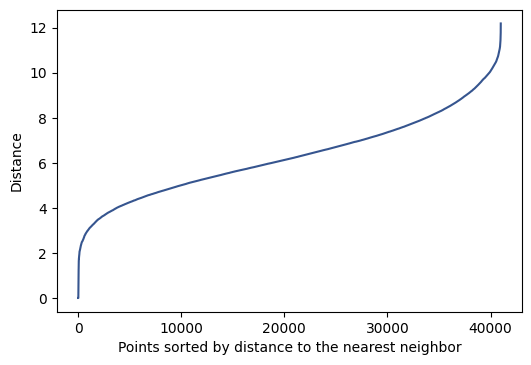
\includegraphics[width=0.7\textwidth]{images/face/dbscan-parameter-estimation-0.png}
		\caption{TODO}
		\label{fig:db0}
	\end{figure}
	
	\begin{figure}[ht]
		\begin{subfigure}{.5\textwidth}
			\centering
			% include first image
			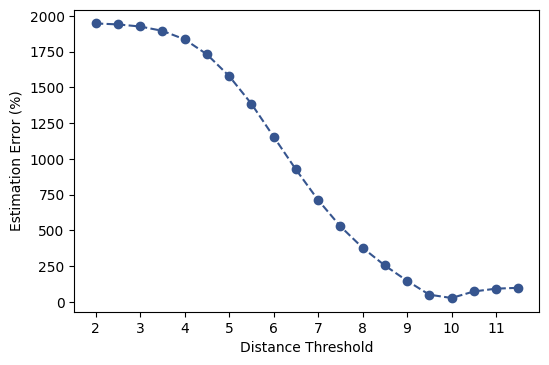
\includegraphics[width=.9\linewidth]{images/face/dbscan-parameter-estimation-1.png}  
			\caption{TODO}
			\label{fig:db-sub-first}
		\end{subfigure}
		\begin{subfigure}{.5\textwidth}
			\centering
			% include second image
			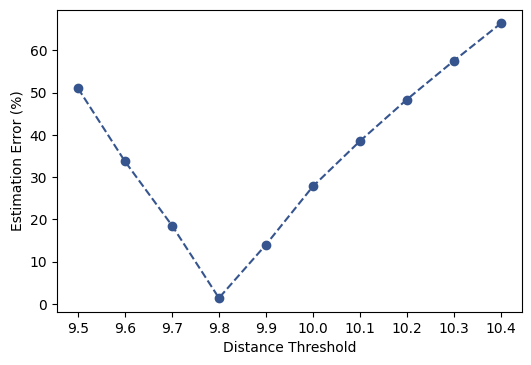
\includegraphics[width=.9\linewidth]{images/face/dbscan-parameter-estimation-2.png}  
			\caption{TODO}
			\label{fig:db-sub-second}
		\end{subfigure}
		\caption{TODO}
		\label{fig:db12}
	\end{figure}
	% --------------------------------------------------------------------------------------
	
	Although CW is itself a parameter-free, unsupervised clustering algorithm, it requires a weighted graph as input. As mentioned in section X, in order to generate this graph a threshold value for distance is required. We explore different values for the distance threshold and again select the value that produces the lowest estimation error. Based on the results (Figure \ref{fig:cw12}), we select a distance threshold value of 72.
	
	% CW Param images ------------------------------------------------------------------
	\begin{figure}[ht]
		\begin{subfigure}{.5\textwidth}
			\centering
			% include first image
			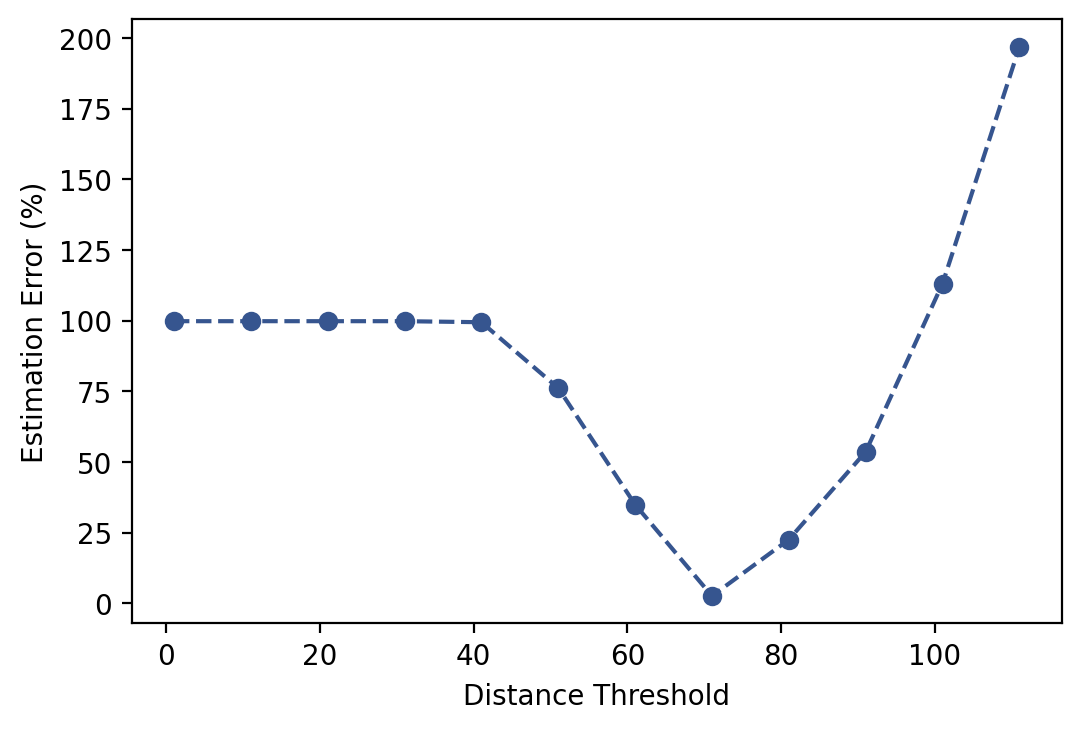
\includegraphics[width=.9\linewidth]{images/face/cw-parameter-estimation-1.png}  
			\caption{TODO}
			\label{fig:cw-sub-first}
		\end{subfigure}
		\begin{subfigure}{.5\textwidth}
			\centering
			% include second image
			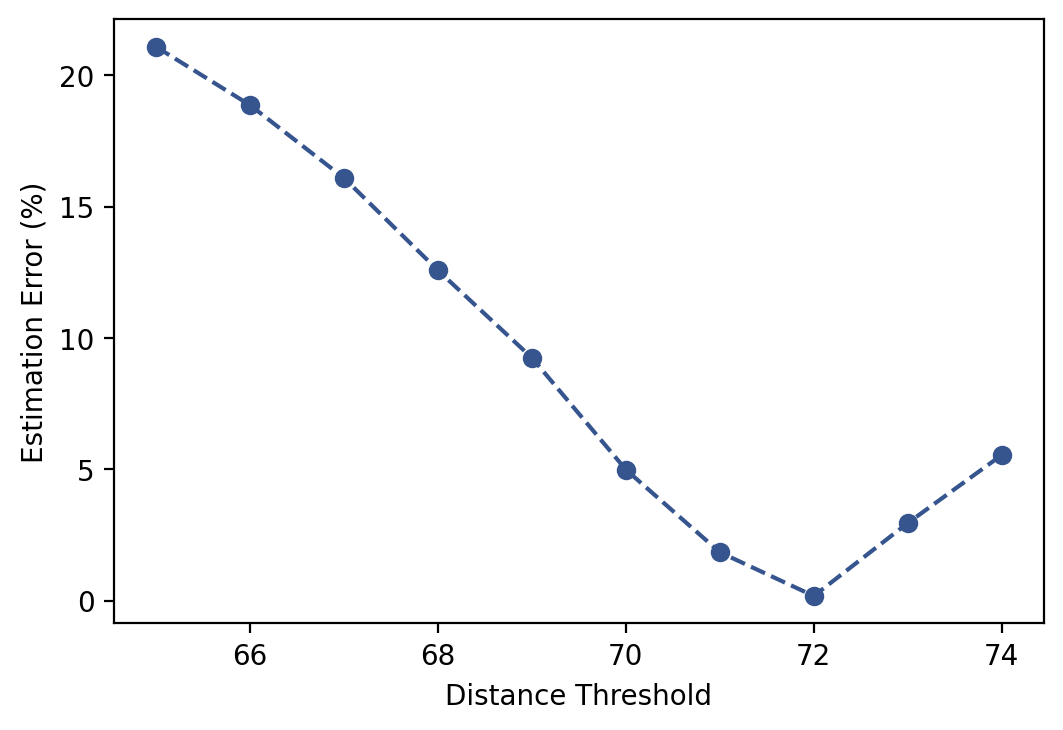
\includegraphics[width=.9\linewidth]{images/face/cw-parameter-estimation-2.png}  
			\caption{TODO}
			\label{fig:cw-sub-second}
		\end{subfigure}
		\caption{TODO}
		\label{fig:cw12}
	\end{figure}
	% --------------------------------------------------------------------------------------
	
	\section{Test 1}
	The first misuse indicator we consider highlights possible wide-scale surveillance, in which a customer is using the facial recognition system to process the faces of a large number of individuals. This could indicate large-scale biometric processing of individuals, which could suggest inappropriate population monitoring. This indicator examines the logs of a facial recognition service to determine the number of different faces a customer processes.
	
	\subsection{Method}
	We generate usage logs that contain entries from both the LFW and ColorFeret datasets. In total this merged dataset contains 24517 images of 6743 people.
	
	Two types of logs are generated. With \textbf{fixed logs}, we first explore the effects of varying the number of different faces in each log, while fixing the size of the overall log. On the other hand with \textbf{varied logs} we explore the effects of logs size and fix the number of faces present and vary the size of the log. To generate the required number of entries, some encodings in the log are repeated.
	
	\subsection{Results}
	% Mention hidden overhead of putting the data into graph form 
	
	\section{Test 2}
	The second misuse indicator we consider highlights potential small-scale surveillance, or stalking. Here the misuse indicator would flag instances where a customer was processing an unusually large number of images of a single person.
	
	\subsection{Method}
	As before, we generate usage logs that contain entries from both the LFW and ColorFeret datasets. We explore a variety of log sizes where each log contains a disproportionate $(\approx 10\%)$ number of images of a single individual. 
	
	\subsection{Results}
	
	\section{Summary}
	% 3-4 sentences describing a summary of the chapter
	
	\chapter{Hate Speech Detection}
	The automated analysis of natural language, such as speech and text, by machines is known as natural language processing (NLP). Driven by the dramatic increase in smart device use, as well as the transition to customer service chatbots, NLP has quickly become one of the most heavily researched subjects in the field of AI. 
	
	In the past, training and implementing machine learning models for projects was a time-consuming process that involved a team of specialists and costly infrastructure. However, the growing demand for such applications prompted major service providers, including Google, AWS, Azure and IBM, to offer pre-built NLP models as-a-service. This significantly decreased workload and infrastructure costs for the average user. For this task we consider the potential for the misuse of these NLP models for processing hate speech.
	
	\section{Motivation}
	According to the 2020 NLP industry survey, over three-quarters of NLP users utilise a cloud NLP service \cite{2020NLPS66:online}, with Google Cloud the most popular. Despite the global COVID-19 pandemic, respondents indicated that spending on NLP had still consistently increased, with 31\% reporting that their budget was at least 30\% higher, in comparison to 2019. 
	
	AIaaS providers offer accessible web-based APIs for powerful NLP models, trained on huge document corpuses, for tasks such as sentiment analysis, speech synthesis and content classification. In general, an API request will specify the desired model along with the raw data, and the service provider will process the request and return the results of the NLP model as a response. An issue can arise when service providers are processing potentially harmful content, in particular hate speech.
	
	According to the Cambridge dictionary, hate speech ‘expresses hate or encourages violence toward a person or group based on something such as race, religion, sex etc’ \cite{HATESPEE16:online}. The rising prevalence of hate speech on social media, as well as the pressing need for effective countermeasures, have attracted substantial investment from governments, businesses, and academics in recent years. In 2016, Facebook, Google, Microsoft, and Twitter signed a code of conduct from the European Union that requires them to review ‘[the] majority of valid notifications for removal of illegal hate speech’ posted on their services within 24 hours \cite{hern2016facebook}.
	
	AIaaS providers have a vested interest in ensuring that their services are used responsibly, both legally and socially. One major driver is reputation; a controversial application developed with these services, such as a racist chatbot, could elicit public backlash and undesirable publicity. AIaaS providers could analyse the data passed to the NLP models to detect those applications early on. The aim of this task is to explore algorithms that can identify instances of potentially harmful material that should be flagged for further investigation.
	
	\section{Challenges}
	The role of detecting hate speech on social media is critical. The unchecked proliferation of hate has the potential to seriously harm society, in particular marginalised people and their communities. However, there are many obstacles to detecting hate speech. 
	
	To begin with, there is a lack of consensus as to what constitutes hate speech. Some researchers, including Ross et al. \cite{ross2017measuring}, believe that a consistent, clear description of hate speech would make hate speech annotations more reliable and easier to do. As a result, hate speech would be easier to detect. Unfortunately however, since the line between hate speech and acceptable free speech is vague, some are hesitant to assign a clear definition. In this research we make use of a variety of existing hate speech datasets with a range of requirements and definitions for hateful speech. 
	
	The context-dependent nature of the classification task also massively contributes to the difficulty. In this scenario, we would rather be overly cautious and flag all possible cases for further investigation. Although the problem of offensive and harmful speech online is serious, hate speech only accounts for a relatively limited portion of overall discourse. As a result, the available datasets are incredibly unbalanced. Although the existing datasets reflect this balance, the actual percentage of hate speech present is larger to allow for effective model training. 
	
	\section{Text Classification Approaches}
	A vast number of techniques have been developed for automatically detecting hate speech online. In tandem with the perceived importance of the task, the field of hate speech detection has been steadily increasing since its conception in 2012 \cite{warner2012detecting}. In this paper we present lexicon as well as machine learning based approaches to the task of hate speech detection.
	
	\subsection{Lexicon-based}
	With lexicon-based approaches we determine whether a piece of text is harmful, based on the words or phrases that occur in the text. A lexicon-based approach is simple, easy to modify and does not rely on a labelled training dataset. It can handle apparent profanity with ease, but not the nuance of expression in hate speech.
	
	For this task, we use a hate speech lexicon assembled by Hatebase.org, the world’s largest online repository of terms and phrases identified as hate speech. The lexicon is regularly updated, with users able to log on and add examples of hate speech from their communities. As of writing Hatebase comprises $3,877$ terms that cover 98 languages. For this project we consider the $1,556$ English terms. Documents containing any of these terms are flagged for further review.
	
	\subsection{Machine Learning Approaches}
	The use of artificial intelligence (AI) technologies to identify harmful material has been the subject of extensive academic and industrial research \cite{macavaney2019hate}. In this section we explain three supervised machine learning approaches to hate speech detection, Naive-Bayes, logistic regression and support vector machines. 
	
	The raw documentents are converted into a matrix of TF-IDF features (see section X). We first evaluate the performance of the three machine learning models using the TF-IDF features alone. We then evaluate the performance of the machine learning models using the sentiment of the document as an additional feature during classification. In this section we cover the three algorithms as well as the mechanism used to determine the sentiment of each document. 
	
	\subsubsection{Naive-Bayes}
	The Naive-Bayes classifier is a probabilistic based classification algorithm, derived from Bayes’ rule
	% Bayes' Rule
	\[P( \, c \, | \, d \,)=\frac{P(c)P(\, d \, | \, c \,)}{P(d)}\]
	and assumes conditional independence of features \(f_i\) given document \(d\)'s class,
	% Naive Bayes' rule
	\[P_{NB}(\, c \, | \, d \,)= \frac{P(c)
		(\prod_{i=1}^{m}P(\, f_i \, | \, c \,)^{n_i(d)})}	% numerator	
	{P(d)}\]												% denominator	 
	Naïve-Bayes assigns \(d\), with feature vector \(\vec{d}\), the most probable class \(\hat{c}\),	
	% Predicting a class
	\[ \hat{c} = \argmax_{c \in \mathcal{C}} P( \,c \, | \, \vec{d} \,)
	= \argmax_{c \in \mathcal{C}} P(c)\prod_{i=1}^{m} P( \, f_i \, | \, c \,)\]
	Despite the oversimplified assumptions, Naive-Bayes works well in many real-world applications \cite{rish2001empirical}. 
	
	
	\subsubsection{Logistic Regression}
	Logistic regression is a fundamental classification technique. It uses the logistic function to model the conditional probability and explain the relationship between one dependent variable and one or more independent variables.  
	
	\subsubsection{Support Vector Machines}
	Support Vector Machines (SVM) are a generalisation of simple maximal margin classifiers, formally defined by a separating hyperplane. Given labelled training data in the form of $n$-dimensional vectors, the algorithm outputs an optimal $(n-1)$-dimensional hyperplane, maximising the margin between vectors in each class. The predicted class of a test instance is determined by which side of the hyperplane it falls on.
	
	\subsubsection{Sentiment Analysis}
	Sentiment analysis is the practice of ‘computationally' deciding whether a piece of writing is positive, negative, or neutral. It is assumed that the majority of hate speech exhibits a higher degree of negative polarity, in comparison to non hate speech. We compute the sentiment on the raw data using an implementation of a sentiment analyser. VADER (Valence Aware Dictionary and sEntiment Reasoner) is a lexicon and rule-based sentiment analysis tool that is uniquely tailored to sentiments expressed in social media \cite{hutto2014vader}.
	
	\section{Experimental Setup}
	We conduct experiments to explore the potential of different hate speech detection algorithms. The experiments were conducted on a personal computer, specifically the  Dell XPS - 8th gen Intel Core i7, 16GB Ram, 500GB SSD, running Windows.
	
	\subsection{Datasets}
	In their 2020 paper, Derczynski et al. systematically review over 60 publicly available English-language datasets created to train abusive language classifiers \cite{vidgen2020directions}. For this task we consider four of these labelled datasets, Davidson et al. \cite{davidson2017automated}, Founta et al. \cite{founta2018large}, Waseem \& Hovy \cite{waseem-hovy:2016:N16-2}, and Stormfront \cite{waseem-hovy:2016:N16-2}.
	
	The Davidson et al. dataset features tweets labelled by a minimum of three annotators. As per previous research with this dataset, we consider only tweets for which a majority of annotators (at least half) agree on a label. The Hatebase lexicon was used to extract a set of twitter users that have tweets containing these specific terms. Tweets are randomly sampled from the timelines of these users. The authors use crowdsourcing to annotate the tweets.
	
	Waseem and Hovy also provide a dataset from Twitter. This time the authors themselves annotated the tweets. Once labelled, they had a gender studies expert review the annotations. The original Founta et al. dataset contains around 100K tweets with one of four labels. Unfortunately, due to deleted tweets or suspended user accounts, we were only able to crawl $16895$ tweets out of the $99,996$ tweets IDs. The tweets were labelled by 20 crowdworkers. Unlike the previous datasets that contain data from Twitter, the Stormfront dataset contains posts from a white supremacist forum. Here the posts are annotated at sentence level.
	
	\begin{table}[htbp]
		\centering
		\begin{tabular}{|c|c|l|l|}
			\hline
			Dataset         & Source       & \multicolumn{1}{c|}{Label}                                                  & \multicolumn{1}{c|}{Count}                                        \\ \hline
			Davidson et al. & Twitter      & \begin{tabular}[c]{@{}l@{}}hateful*\\ offensive*\\ neutral\end{tabular}     & \begin{tabular}[c]{@{}l@{}}1429\\ 19188\\ 4163\end{tabular}       \\ \hline
			Waseem \& Hovy  & Twitter      & \begin{tabular}[c]{@{}l@{}}sexism*\\ racism*\\ none\end{tabular}            & \begin{tabular}[c]{@{}l@{}}4217\\ 25\\ 12663\end{tabular}         \\ \hline
			Founta et al.   & Twitter      & \begin{tabular}[c]{@{}l@{}}hateful*\\ abusive*\\ spam\\ normal\end{tabular} & \begin{tabular}[c]{@{}l@{}}653\\ 3064\\ 2442\\ 10736\end{tabular} \\ \hline
			Stormfront      & Online forum & \begin{tabular}[c]{@{}l@{}}hate*\\ relation\\ skip\\ neutral\end{tabular}   & \begin{tabular}[c]{@{}l@{}}1196\\ 168\\ 73\\ 9507\end{tabular}    \\ \hline
		\end{tabular}
		\caption{Summary of the hate speech datasets (*denotes harmful labels)}
		\label{tab:hatespeech_datasets}
	\end{table}
	
	Table \ref{tab:hatespeech_datasets} contains a summary of the datasets. We use Davison et al. to train the hate speech classifiers. The remaining datasets are merged and used to generate usage logs and evaluate the performance of the different approaches.
	
	\subsection{Preprocessing}
	The usage logs we examine for this task describe data that could be passed to an NLP cloud service and contain raw text. Before passing the data as input to the classification models, several preprocessing steps are required to clean the data. Preprocessing is performed on both the training (Davison et. al) and testing datasets.
	
	Preprocessing of the datasets involved, tokenizing, stemming, stop-word and punctuation removal and case folding. Tokenization converts each document into a list of words, or tokens. The Porter stemmer then converts each of the words into their root forms \cite{porter1997readings}. We remove stopwords using the Natural Language Toolkit (nltk) library that contains 2,400 stopwords for 11 languages. Cleaning also involves the removal of punctuation, additional whitespaces, links and usernames.
	
	The aim of this misuse indicator is to flag any instances of harmful speech. As a result, we model hate speech detection as a binary classification task such that a document either contains harmful speech and requires review, or does not. The asterisk symbols in table X denote which classes in each dataset we consider `harmful’
	
	Term Frequency - Inverse Document Frequency (TF-IDF) is a feature extraction technique \cite{ramos2003using}. The tf-idf vectorizer converts a collection of raw documents to a matrix of TF-IDF features. In a large text corpus, some words will be very present (e.g. `the’ in English) hence carrying very little meaningful information about the actual contents of the document. Rarer words carry more information; the TF-IDF vectorizer normalizes the counts according to the frequency of the n-gram in question in the whole corpus. The cleaned documents are passed further for feature extraction. We embed words and n-grams (contiguous sequences of n items) with TF-IDF and extract sentiment polarity scores.
	
	\section{Results}
	
	\section{Summary}
	% 3-4 sentences describing a summary of the chapter
	
	%\chapter{Summary and Conclusions} 
	\chapter{Discussion}
	
	
	\appendix
	\singlespacing
	
	\bibliographystyle{unsrt} 
	\bibliography{dissertation} 
	
\end{document}
